\documentclass{article}
\usepackage{tikz}
\usetikzlibrary{shapes.geometric, arrows.meta}

\tikzstyle{startstop} = [rectangle, rounded corners, minimum width=3cm, minimum height=1cm,text centered, draw=black, fill=red!30]
\tikzstyle{process} = [rectangle, minimum width=3cm, minimum height=1cm, text centered, draw=black, fill=orange!30]
\tikzstyle{decision} = [diamond, minimum width=3cm, minimum height=1cm, text centered, draw=black, fill=green!30]
\tikzstyle{arrow} = [thick,->,>=stealth]

\begin{document}

\begin{figure}[h]
    \centering
    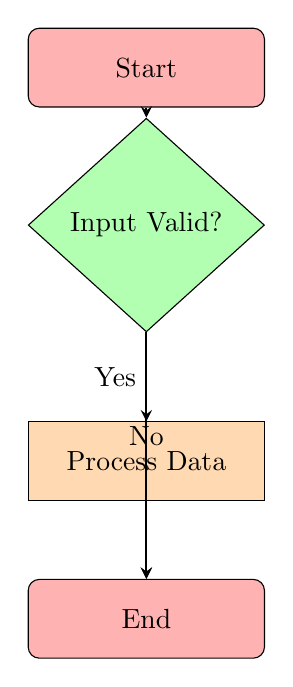
\begin{tikzpicture}[node distance=2cm]
        % Nodes
        \node (start) [startstop] {Start};
        \node (inval) [decision, below of=start] {Input Valid?};
        \node (proc) [process, below of=inval, yshift=-1cm] {Process Data};
        \node (end) [startstop, below of=proc] {End};

        % Arrows
        \draw [arrow] (start) -- (inval);
        \draw [arrow] (inval) -- node[anchor=east] {Yes} (proc);
        \draw [arrow] (inval) -- node[anchor=south] {No} (end);
        \draw [arrow] (proc) -- (end);
    \end{tikzpicture}
    \caption{Flowchart of the Process}
    \label{fig:flowchart}
\end{figure}

\end{document}